%%%%%%%%%%%%%%%%%%%%%%%%%%%%%%%%%%%%%%%%%
% Short Sectioned Assignment
% LaTeX Template
% Version 1.0 (5/5/12)
%
% This template has been downloaded from:
% http://www.LaTeXTemplates.com
%
% Original author:
% Frits Wenneker (http://www.howtotex.com)
%
% License:
% CC BY-NC-SA 3.0 (http://creativecommons.org/licenses/by-nc-sa/3.0/)
%
%%%%%%%%%%%%%%%%%%%%%%%%%%%%%%%%%%%%%%%%%

%----------------------------------------------------------------------------------------
%	PACKAGES AND OTHER DOCUMENT CONFIGURATIONS
%----------------------------------------------------------------------------------------

\documentclass[paper=a4, fontsize=11pt]{scrartcl} % A4 paper and 11pt font size

\usepackage[T1]{fontenc} % Use 8-bit encoding that has 256 glyphs
%\usepackage{fourier} % Use the Adobe Utopia font for the document - comment this line to return to the LaTeX default
\usepackage[english]{babel} % English language/hyphenation
\usepackage{amsmath,amsfonts,amsthm} % Math packages
\usepackage{bm}
\usepackage{lipsum} % Used for inserting dummy 'Lorem ipsum' text into the template
\usepackage{graphicx} % This one is for pictures
\usepackage{sectsty} % Allows customizing section commands
\allsectionsfont{\centering \normalfont\scshape} % Make all sections centered, the default font and small caps
\usepackage{color}

\usepackage{fancyhdr} % Custom headers and footers
\pagestyle{fancyplain} % Makes all pages in the document conform to the custom headers and footers
\fancyhead{} % No page header - if you want one, create it in the same way as the footers below
\fancyfoot[L]{} % Empty left footer
\fancyfoot[C]{} % Empty center footer
\fancyfoot[R]{\thepage} % Page numbering for right footer
\renewcommand{\headrulewidth}{0pt} % Remove header underlines
\renewcommand{\footrulewidth}{0pt} % Remove footer underlines
\setlength{\headheight}{13.6pt} % Customize the height of the header

%\numberwithin{equation}{section} % Number equations within sections (i.e. 1.1, 1.2, 2.1, 2.2 instead of 1, 2, 3, 4)
%\numberwithin{figure}{section} % Number figures within sections (i.e. 1.1, 1.2, 2.1, 2.2 instead of 1, 2, 3, 4)
%\numberwithin{table}{section} % Number tables within sections (i.e. 1.1, 1.2, 2.1, 2.2 instead of 1, 2, 3, 4)

%\setlength\parindent{0pt} % Removes all indentation from paragraphs - comment this line for an assignment with lots of text

%----------------------------------------------------------------------------------------
%	TITLE SECTION
%----------------------------------------------------------------------------------------

\newcommand{\horrule}[1]{\rule{\linewidth}{#1}} % Create horizontal rule command with 1 argument of height

\title{	
\normalfont \normalsize 
\textsc{Columbia University -- Fall 2013} \\ [25pt] % Your university, school and/or department name(s)
\horrule{0.5pt} \\[0.4cm] % Thin top horizontal rule
\huge Machine Learning Homework \#4\\ % The assignment title
\horrule{2pt} \\[0.5cm] % Thick bottom horizontal rule
}

\author{Joe Ellis - jge2105} % Your name

\date{\normalsize\today} % Today's date or a custom date

\begin{document}

\maketitle % Print the title

%----------------------------------------------------------------------------------------
%	PROBLEM 1
%----------------------------------------------------------------------------------------

\section{Problem 1 -- EM Derivation}
In this problem we will derive the Expectation-Maximization algorithm for a mixture of multinomials.
Suppose, that $x$ is represented as a vector such that $x(j) = 1$ if $x$ takes the $j^{th}$ value, and $\sum_j x(j) = 1$.
The distribution of $x$ is described by a mixture of $K$ discrete multinomials such that:

\begin{align}
p(x) = \sum_{k=1}^K \pi_k p(x|\mu_k)
\end{align}

where 

\begin{align}
p(x|\mu_k) = \prod_{j=1}^M \mu_k(j)^{x(j)}.
\end{align}

Where $\pi_k$ is the mixing coefficients, and $\mu_k$ specifies the parameters of the $k^th$ component.
We then must derive the Expectation and Maximization steps to maximize the log-likelihood of an observed data set $\{x_i\}$.

\subsection{Expectation Step}
First we want to calculate what is referred to in EM as the responsibilities of each data point given the mixtures.
To do this we want to find the $p(z_i|x_i;\theta)$, where $z_i$ is the mixture that this data point belongs to.
In this way, we can estimate the likelikhood that each data point was generated by one of the given mixtures, and then weight our estimates in the maximization step accordingly.

\begin{align}
p(z_i|x_i|;\theta) &= \frac{p(x_i|z_i;\theta)p(z_i)}{p(xi)},	\ by Bayes Rule \\
&= \frac{p(x_i|z_i;\theta)\pi_k}{p(xi)} \\
&= \frac{p(x_i|\mu_k)\pi_k}{\sum_{k=1}^K \pi_k p(x|\mu_k)} \\
&= \frac{\pi_k\mu_k^{x_i(j)}}{\sum_{k=1}^K \pi_k\mu_k^{x_i(j)})}. \\
\end{align}

Therefore, we have the responsibilities of each data point, and have calculated how likely each data point was generated from each mixture.

\subsection{Maximization Step}
Now that we have the responsibilities we will in turn now calculate the parameters $\mu_k$ and $\pi_k$ that maximize the log-likelihood function of the seen data.
Let's find the log-likelihood of the data given our hidden variables $\theta$, to do this, we must maximize the general form of the equation below.

\begin{align}
\theta := \underset{\theta}{\operatorname{argmax}}\sum_{i=1}^N \sum_{z_i}(Q_i(z_i)\frac{p(x_i,z_i;\theta)}{Q_i(z_i)}).
\end{align}

In the above equation $Q_i(z_i)$ is the value for each mixture and data point that is calculated using the E-step from above.
In the derivation below we will use the notation $\tau_{k,i}$, where $\tau_{k,i} = Q_i(z_k)$.
Let's refer to the above equation as $l(\theta)$

\begin{align}
l(\theta) &= \sum_{i=1}^N \sum_{k=1}^K \tau_{k,i} log(\frac{p(x_i,z_i;\theta)}{\tau_{k,i}} \\
&= \sum_{i=1}^N \sum_{k=1}^K \tau_{k,i} log(p(x_i,z_i;\theta)) -  \sum_{i=1}^N \sum_{k=1}^K \tau_{k,i} log( \tau_{k,i}) \\
&= \sum_{i=1}^N \sum_{k=1}^K \tau_{k,i} log(p(x_i,z_i;\theta)) -  const \\
&=  \sum_{i=1}^N \sum_{k=1}^K \tau_{k,i} log( \pi_k\prod_{j=1}^M \mu_k(j)^{x_i(j)}) \\
&= \sum_{i=1}^N \sum_{k=1}^K \tau_{k,i} log(\pi_k) + \sum_{j=1}^M log(\mu_k(j)^{x_i(j)}) \\
&= \sum_{i=1}^N \sum_{k=1}^K \tau_{k,i} log(\pi_k) + \tau_{k,i}\sum_{j=1}^M x_i(j) log(\mu_k(j)) \\.
\end{align}

Now that we have derived the log likelihood we must maximize the above equation with respect to the parameters $\mu$ and $\pi$.
However the derivation is not straight forward and we must use laplaclian variables to satisfy the constraints of, $\sum_j \mu_k(j) = 1$ and $\sum_k \pi_k = 1$.

Therefore, let's do the derivation.
We set the derivative with respect to $\mu_k(j)$ and the constraints with laplace variable $\lambda$ to zero and solve.

\begin{align}
\frac{\partial l(\theta)}{\partial \mu_k(j)} &=\frac{\partial}{\partial \mu_k(j)}  \sum_{i=1}^N \sum_{k=1}^K \tau_{k,i} log(\pi_k) + \tau_{k,i}\sum_{j=1}^M x_i(j) log(\mu_k(j)) - \sum_{k=1}^K \lambda_k (\sum_{j=1}^M \mu_k(j) -1) \\
&=  \sum_{i=1}^N  \tau_{k,i} \frac{1}{\mu_k(j)} - \lambda_k = 0. \\
\end{align}

Thus, 

\begin{align}
\mu_k(j) =  \frac{\sum_{i=1}^N x_i(j) \tau_{k,i}}{\lambda_k}.
\end{align}

Plugging $\mu_k(j)$ back into the equation, $\sum_{j=1}^M \mu_k(j) -1)$ gives us the equation for $\lambda_k$ below,

\begin{align}
\lambda_k = \sum_{i=1}^N \sum_{m=1}^M \tau_{k,i} x_i(m).
\end{align}

So therefore we have the update for our $\mu_k(j)$ as, 

\begin{align}
\mu_k(j) = \frac{\sum_{i=1}^N \tau_{k,i} x_i(j)}{\sum_{i=1}^N \sum_{m=1}^M \tau_{k,i} x_i(m)}
\end{align}

Similarly, we can derive the value for the other parameter $\pi_k$, with laplacian constraints.

\begin{align}
\frac{\partial l(\theta)}{\partial \pi_k} &=\frac{\partial}{\partial \pi_k}  \sum_{i=1}^N \sum_{k=1}^K \tau_{k,i} log(\pi_k) + \tau_{k,i}\sum_{j=1}^M x_i(j) log(\mu_k(j)) - \lambda (\sum_{k=1}^K \pi_k -1) \\
&=  \sum_{i=1}^N  \tau_{k,i} \frac{1}{\pi_k} - \lambda = 0. \\
\end{align}

Thus, 

\begin{align}
\pi_k =  \frac{\sum_{i=1}^N \tau_{k,i}}{\lambda}.
\end{align} 

Plugging $\lambda$, back into the constraint equation, $\sum_{k=1}^K \pi_k -1)$, we solve for lambda, 

\begin{align}
\lambda &= \sum_{i=1}^N \sum_{k=1}^K \tau_{k,i} \\
& = N.
\end{align}

So, therefore we have the update for our mixing coefficients ($\pi_k$) as,

\begin{align}
\pi_k = \frac{\sum_{i=1}^N \tau_{k,i}}{N} \\
\end{align}

Therefore, we have derived the entire EM algorithm for a mixture of multinomials.


%----------------------------------------------------------------------------------------
%	PROBLEM 2
%----------------------------------------------------------------------------------------
\section{Problem 2}

\subsection{Mixtures of Gaussians}
Using the code provided to us in the tutorial section of the class website we were able to perform EM on a mixture of gaussians on two datasets.
The figures generated from the EM algorithm and the gaussian distributions found are superimposed over the data points.

Figures \ref{fig:datasetA} and \ref{fig:datasetB} show the results of the EM calculation.

\begin{figure}
\centering
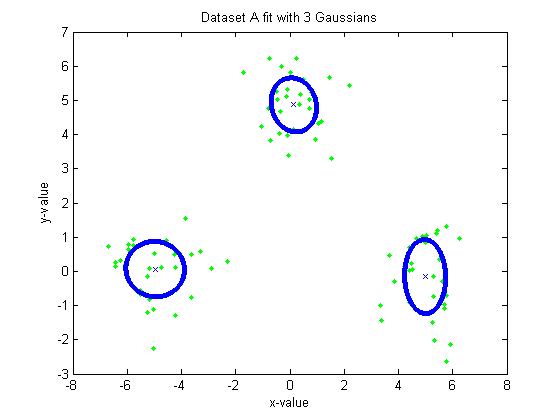
\includegraphics[width=0.5\textwidth]{datasetA.png}
\caption{EM result on dataset A using 3 Gaussian distributions}
\label{fig:datasetA}
\end{figure}

\begin{figure}
\centering
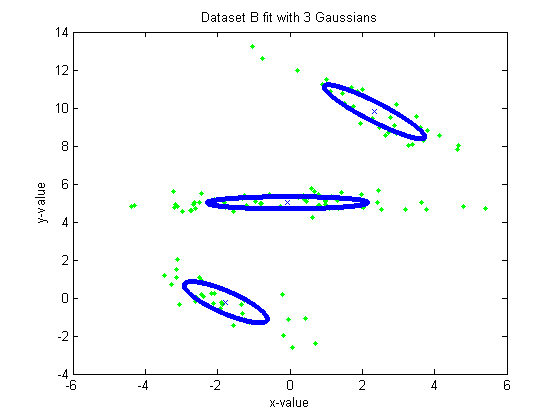
\includegraphics[width=0.5\textwidth]{datasetB.png}
\caption{EM result on dataset B using 3 Gaussian distributions}
\label{fig:datasetB}
\end{figure}

\subsection{Mixtures of Multinomials}
In this section we explore using the derivation provided in section 1 to create a mixture of multinomials model to differentiate between plays written by Shakespeare and Middleton.
We have 9 plays written by Shakespeare and 9 plays written by Middleton, and we will try to classify how we well we can seperate the two using multiple mixture models.


%----------------------------------------------------------------------------------------
%	PROBLEM 3
%----------------------------------------------------------------------------------------
\section{Problem 3}




\end{document}